\subsection{Korrespondenzen elementarer Signalformen}

\subsubsection{Zusammenfassung wichtiger Korrespondenzen}

\begin{table}[h]
    \centering
    \begin{tabular}{|c|c|c|}
        \hline
        Abtastwerte $x[k]$ & Z-Transformierte $X(z)$ & Konvergenzbereich \rule{0pt}{0.5cm} \\
        \hline 
        Dirac-Impuls $\delta[k]$ & $1$ & $|z| \in \mathbb{R}$\rule{0pt}{0.5cm} \\
        \hline
        Sprungfunktion $\epsilon[k]$ & $\frac{z}{z-1}$ & $|z| > 1$\rule{0pt}{0.5cm} \\
        \hline
        $\epsilon[k] \cdot k$ & $\frac{z}{(z-1)^2}$ & $|z| > 1$\rule{0pt}{0.5cm} \\
        \hline
        $\epsilon[k] \cdot a^k$ & $\frac{z}{(z-a)^2}$ & $|z| > a$\rule{0pt}{0.5cm} \\
        \hline
        $\epsilon[k] \cdot e^{-ak}$ & $\frac{z}{(z-e^{-a})}$ & $|z| > e^{-a}$\rule{0pt}{0.5cm} \\
        \hline
        $\epsilon[k]\cdot sin(\omega k T)$ & $\frac{z\cdot sin(\omega T)}{z^2 - 2\cdot cos(\omega T)\cdot z + 1}$ & $|z| > 1$ \rule{0pt}{0.5cm}\\
        \hline
        $\epsilon[k]\cdot cos(\omega k T)$ & $\frac{z\cdot cos(\omega T)}{z^2 - 2\cdot cos(\omega T)\cdot z + 1}$ & $|z| > 1$ \rule{0pt}{0.5cm}\\
        \hline
    \end{tabular}
    \caption{Korrespondenzen elementarer Signalformen\cite[S.218]{book4}}
    \label{tab:ZT_Korrespondenzen}
    
\end{table}

Im Folgenden werden drei dieser Korrespondenzen beispielhaft näher betrachtet, um besser zu verstehen, wie diese zustande kommen.

 \subsubsection{Dirac-Impuls}
 \begin{minipage}[c]{0.45\textwidth}  $\delta[k] = \begin{cases}
        1 &, k=0 \\
        0 &, k \neq 0
    \end{cases}$
    \end{minipage}
    \begin{minipage}[c]{0.45\textwidth}
        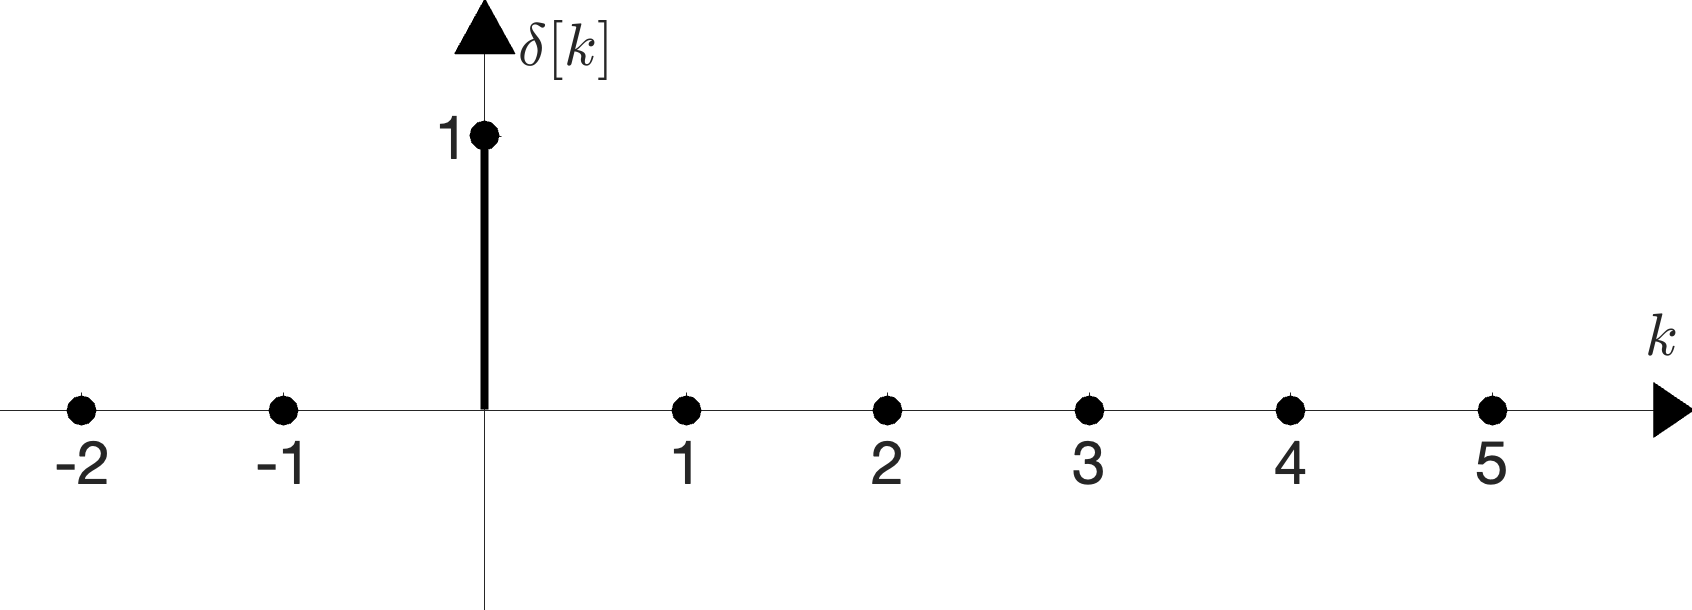
\includegraphics[width=\textwidth]{Anlagen/ZT_Impuls.png}
    \end{minipage}
    \begin{align}
        &\mathcal{Z}\{\delta[k]\} = \sum_{k=0}^{\infty}\delta[k]z^{-k} = 1\cdot z^0 = 1 \\
        &\delta[k] \TransformHoriz 1 \text{ mit } |z| \in \mathbb{R}
    \end{align}

\subsubsection{Sprungfunktion}
    \begin{minipage}[c]{0.45\textwidth} $\epsilon[k] = \begin{cases}
        1 &, k \geq 0 \\
        0 &, k < 0
        \end{cases}$
    \end{minipage}
    \begin{minipage}[c]{0.45\textwidth}
        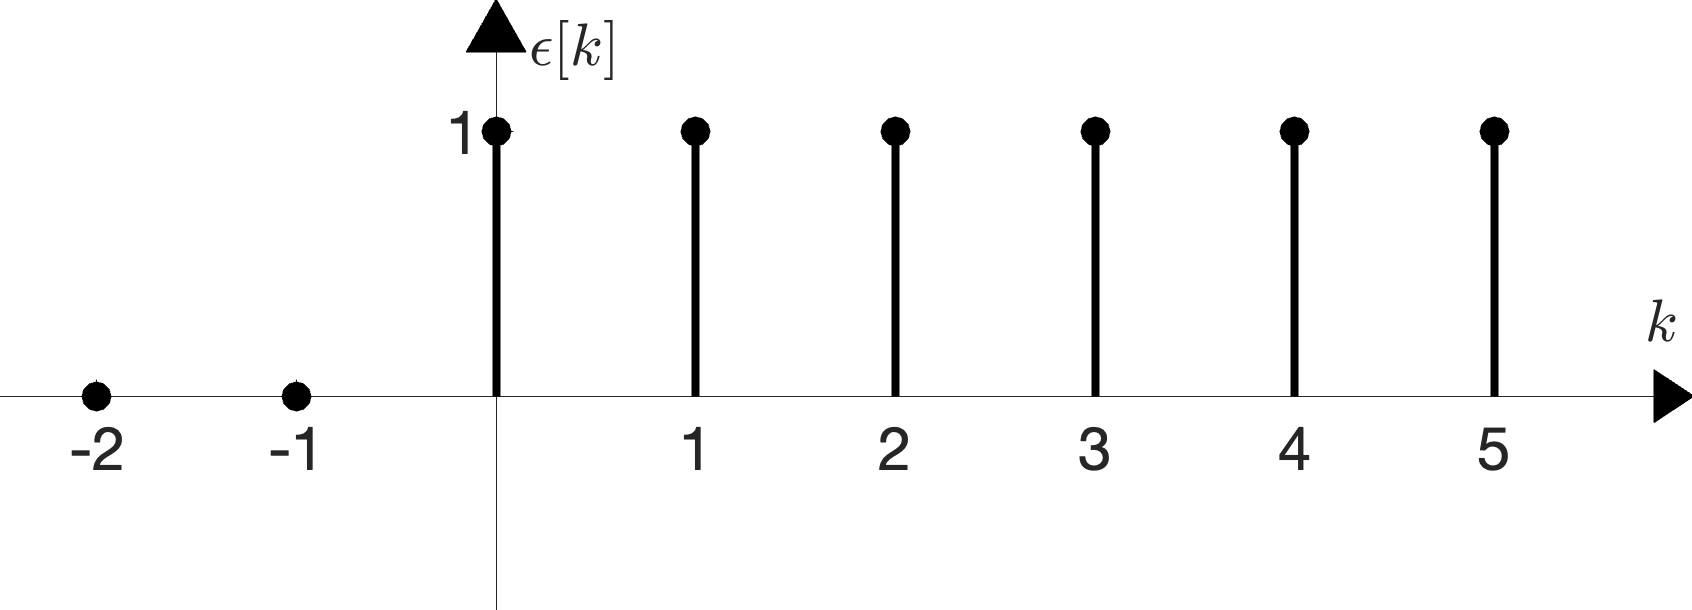
\includegraphics[width=\textwidth]{Anlagen/ZT_Einheitssprung.png}
    \end{minipage}
    \begin{align}
        &\mathcal{Z}\{\epsilon[k]\} = 1 + \frac{1}{z} + \frac{1}{z^2} + ... = \frac{1}{1-\frac{1}{z}} = \frac{z}{z-1}  \\
        \notag
        &\text{Dieser Ausdruck entspricht der geometrischen Reihe, die nur für } |\frac{1}{z}| < 1 \text{ konvergiert:}\\
        &\epsilon[k] \TransformHoriz \frac{z}{z-1} \text{ mit } |z| > 1
    \end{align}
    

\subsubsection{Cosinus}
Zuletzt wird noch die etwas komplexere Korrespondenz der abgetasteten Sinusfunktion $\epsilon[k]\cdot sin(\omega k T)$ hergeleitet:





